
\documentclass[conference]{IEEEtran}
\usepackage{cite}

\usepackage{graphicx}
\usepackage{amsmath}        % extensions for typesetting of math
\usepackage{amsfonts}       % math fonts
\usepackage{amsthm}         % theorems, definitions, etc.
\usepackage{amssymb}

%\usepackage{fancyvrb}       % improved verbatim environment
 %\usepackage{subfig}

%\bibliographystyle{iopart-num}
%\usepackage{iopams}
%\newcommand{\REVTeX}{REV\TeX}
%\usepackage{bm}
\usepackage{cleveref} 

\graphicspath{ {./img/} }
\renewcommand\IEEEkeywordsname{Keywords}


\title{Magnetic and Geometric Properties of the Ising Model on Lattice Random Walks}

\author{Ilya Pchelintsev\\
The Department of Applied Mathmatics\\
National Research University "Higher School of Economics"\\
The Moscow Institute of Electronics and Mathematics\\
Moscow, Russia\\
iipchelintsev@edu.hse.ru}

\begin{document}
\maketitle

%\address{National Research University Higher School of Economics, 101000 Moscow, Russia}


\begin{abstract}
The study focuses on a model on a magnetic polymer chain with closely interacting Ising spins on a lattices with different numbers of dimensions d: square and triangular with d=2, and cubic with d=3. The studied model has dynamic disorder for both spins and conformations, and fixed length of a chain. The shape factors of conformations are considered as geometrical critical observables which can correlate with aspect ratio as a parameter of regular Ising model. The binder cumulant of both models in their respective critical areas with same shape factors are expected to be equal. The mean fraction of monomers on a chain with fixed number of neighbors (or bulks) are considered as a geometric measure of compaction of conformation. Using Monte-Carlo methods in Worm-Algorithm, we compare these measures between chains with respective spin-to-spin coupling constant J in lattices having equal number of highest possible number of monomers. 
\end{abstract}

\begin{IEEEkeywords}
Statistical Physics, Ising model, phase transition, Monte Carlo simulations, shape factors, lattice models
\end{IEEEkeywords}


\section{Introduction}

The model of self-avoiding walks is one of the extensively studied examples of linear polymers. 
Moreover, it is the simplest model to study critical behaviour while other models of polymer chains have different states in the thermal equilibrium in various solvent conditions. 
By adding interaction between nearest neighbors of monomers of the walk, we are enabled to study the phase transition fixed between solvent conditions, so the given polymer in the thermal equilibrium becomes extended in the good-solvent conditions and collapses in the poor-solvent one. 
This tricritical nature was described in \cite{Gennes1979}.

The impact of close-range interaction was studied precisely in models of magnetic polymers, where interaction between monomers became more complex after each monomer carried a spin and the strength of the nearest neighbors coupling became variable. 
This is the so-called Ising Model on a SAW conformation. 
In \cite{Garel1999}, the model was complicated by adding the external magnetic field and all conclusions about magnetic properties were made by comparing with the mean-field model. 
However, there are some geometric properties whose impact on magnetic properties is not clear while their studying may require more brute methods.

In the previous studies \cite{faizullina2021critical}, it was established that the Ising model on the self-avoiding walk conformations (SAWs) has a continuous type of phase transition. 
In this work, we continue to study geometric properties of this model and compare them with "parent" models and their modifications, such as the Ising model on the rectangular lattice, considered in \cite{Selke2006}, and two-dimensional interacting self-avoiding walks exactly in their respective critical regions. 
One of the suggestions is that models with similar geometric properties will also have the same magnetic properties, which can be observed while comparing values of Binder cumulants in the $\theta$-transition of models with the equal values of asphericities.

The rest of the paper is structured as follows. 
Section 2 summarizes the main related work and the previous results in this area. 
Section 3 describes the reseacrhed models, their main geometric and magnetic observables and the simulation methods. 
Sections 4 is divided in two parts, each on them presents the results of the two main directions of the work: the comparison the Ising-ISAW and the regular Ising models in critical areas and the research of the local coordination number in the Ising-ISAW model across several lattice modifications.
The conclusions and the future work are summarized in Section 5.


\section{Literature Review}

There are numerous studies of self-avoiding walk models with different interacting mechanisms. 
Some approaches have focused on critical behaviour of two-dimensional SAW models, by observing the geometrical properties \cite{Caracciolo2011, owczarek2000first, arkin2013gyration}. 
Researchers studied several shape factors, such as average asphericity and size ratios, which are essential in hydrodynamics, by using Monte-Carlo statistical methods. 
They have verified their computations by mean-field theory, widely used in low-dimensional models. 
As a result, they determined an elliptic average shape of the two-dimensional walks and calculated the average ratio of the two axes in the critical area.
Another area of growing interest the critical behaviour of lattices with more available connections between single monomer, such as cubic and triangle Ising-ISAW \cite{Foster2021} and ISAW \cite{Tesi1996, Privman1986} models. 
A number of approaches presented outer-interacting models, designed for hydrodynamics processes \cite{LivneSAW1988, madras1988pivot}. 
A variety of researched lattices prompts studying still underresearched universality of the properties among different models and lattices, particularly geometric ones, which is researched in this study. 
One of the backbone directions of the work is the comparison of geometrical properties of Ising-ISAW model and ISAW model on several lattices, such as square, triangle and cubic ones.

With the significant development of technical characteristics of supercomputers, it became possible to simulate much longer conformations. 
It also paved the way for more accurate research of approximate behaviour of infinite-sized conformations, so it is closer to research of the polymers of the real size. 
Some approaches have already estimated the scaling of the geometrical properties \cite{owczarek2008scaling}. 
Researchers have determined the linear scaling of atmosphere probability of non-interacting SAWs and by linear regression, have calculated the asymptotic limits. 
In this work, the particular attention is paid to analysis of the behaviour of more specific to the model properties. 
The researched geometrical properties of Ising-ISAW models are the local coordination number as a fraction of the monomers with fixed number of neighbours and the atmosphere of the walks. 
The regression methods were required to estimate linear and non-linear scaling coefficients.

\section{Models and Methods}


The paper considers several models: the first one is Ising model on interacting self-avoiding walk from Ref. \cite{faizullina2021critical}, on three different lattices: 2D-square lattice, 3D-square lattice and 2D-triangle lattice. The main difference between square and triangle lattice is two additional diagonal monomers on lattice determined as nearest. This work considers the case of lack of outer magnetic field, the Hamiltonian of the model of fixed conformation $u$ with length $N$ and strength of nearest-neighbors interaction $J$ reads:

\begin{equation}\label{H_Ising_ISAW}
  H_{u, N, \{\sigma\}} = - \sum_{\langle i,j \rangle} J  \sigma_{i}  \sigma_{j},\ \ i,j \in u,\ |u| = N
\end{equation}

The summation runs through spins involved in conformation and only with the nearest neighbors. 

The second model considered in this paper is the Ising model on the rectangular lattice from the Ref.\cite{Selke2006}. Simulated lattices has $L \times rL$ spins and the Hamiltonian is calculated through interaction between all spins and their nearest neighbors respectively:

\begin{equation}\label{H_Ising_Rectan}
  H_{L, r, \{\sigma\}} = - \sum_{\langle i,j \rangle} J  \sigma_{i}  \sigma_{j}
\end{equation}

Here the $i$-th spin of the lattice has a pair of coordinates from $[1..L] \times [1..rL]$. For comparing magnetic properties of models with similar geometric ones, the shape factors are considered, such as gyration tensor of system with $N$ points $w_{i}$ \cite{Caracciolo2011}:

\begin{equation}\label{eq:Ten_G1}
    Q_{N,\alpha\beta} = \frac{1}{N} \sum^{N}_{i=1}(w_{i,\alpha} - w_{c, \alpha})(w_{i,\beta} - w_{c, \beta})
\end{equation}

where $N$ is length of the system (number of monomers in conformations of Ising-ISAW models or number of spins in the lattice in rectangular Ising), and  $w_{i, \alpha},w_{i, \beta}$ are the coordinates of $i$-th point of conformation. $w_{c, \alpha},w_{c, \beta}$ are coordinates of the center of system (so, $Q_{N, xx}$ and $Q_{N,yy}$ can be defined as mean squares of coordinates of the points of the model in the cartesian coordinate system with the center in the center of model). Eugen values $q1$, $q2$ of given tensor can be interpreted as $Q_{N, xx}$ and $Q_{N,yy}$ in the coordinate system of eugen vectors, or more important - as square of semi-axes of ellipse of inertia of given system. The proportion of them for systems with length $N$ will be \cite{Caracciolo2011}: 

\begin{equation}
    r = \sqrt{\frac{\langle q_{1}\rangle_{N}}{\langle q_{2} \rangle_{N}}}
\end{equation}

Eugen values $q1$, $q2$ are also used in enumerating another important shape factor - mean asphericity \cite{Caracciolo2011}:

\begin{equation}
\label{eq:Asphericity}
    \mathcal{A} = \left\langle \frac{(q_{1} - q_{2})^{2}}{(q_{1} + q_{2})^{2}} \right\rangle_{N}
\end{equation}

The compared magnetic property of our models is the fourth order cumulant of the magnetization or the Binder cumulant, defined as \cite{Binder1981_Ising}:

\begin{equation}
\label{eq:Cumulant}
U_{4} = 1 - \frac{\langle m^{4} \rangle}{3 \langle m^{2} \rangle^{2}}
\end{equation}

Where $\langle m^{4} \rangle$ and $\langle m^{2} \rangle$ are mean fourth and second order of mean magnetization per spin respectively.

It is also necessary to determine the mean proportion of monomers with fixed number $i$ of nearest neighbors $\langle n_{i} \rangle$, which is counted directly for every monomer in every simulated conformation of walk.

One of the aims is to compare models in their respective critical regions. For each structure, critical temperatures of Ising models are known as:

\begin{table}[h]
    \centering
    \begin{tabular}{|c|c|c|}
        \hline
        Structure & lattice & $J_{c}$ \\ \hline
        ISAW conformation & Square & $0.8340(5)$\cite{faizullina2021critical} \\ \hline
        ISAW conformation & Cubic & $0.5263 \pm 0.055$\cite{Foster2021}\\ \hline
        Regular lattice & Rectangular & $\ln{(1 + \sqrt{2}) / 2}$\cite{Onsager}\\ \hline
    \end{tabular}
    \label{tab:Ising_T_c}
    \medskip
    \caption{Known values of critical temperature of different modifications of Ising-ISAW model and normal Ising on the rectangular lattice}
\end{table}

\begin{table}[h]
    \centering
    \begin{tabular}{|c|c|}
        \hline
        lattice & $T_{c}$ \\ \hline
        Square & $0.6673(5)$ \cite{Caracciolo2011} \\ \hline
        Cubic & $0.2779 \pm 0.0041$\cite{Tesi1996} \\ \hline
        Triangle & $ 0.405 \pm 0.07$\cite{Privman1986} \\ \hline
    \end{tabular}

    \label{tab:ISAW_T_c}
    \medskip
    \caption{Known values of critical temperature of different modifications of ISAW model}
\end{table}

\section{Results}

\subsection{Mean Asphericity and Critical Cumulant}

The mail goal of this section is to learn how magnetic properties of Ising-like models depend on their geometrical ones and to determine their comparability in the critical region, where dependence of model observables from the length of conformation $N$ is the weakest. 
The idea is to compare critical cumulants $U_{4}$ \eqref{eq:Cumulant} of both models of Ising having equal asphericities. 
Both models are considered to have open boundary conditions (OBC). 
To the best of the author’s knowledge, in the Ising model on rectangular lattice shape factors like aspect ratio $r$ are the parameters, not observable values. 
Therefore, it became possible to find value of the aspect ratio of lattice for any asphericity $\mathcal{A}$ \eqref{eq:Asphericity} (see \cref{fig:A_r}). 
For rectangular lattice, the leading correction term to the asphericity behave like $A^{*}(r) - A(r, L) \propto 1 / L^{2}$. 
Moreover, the value of Binder cumulant in Rectangular Ising in critical region depends on aspect ratio $r$ \cite{Selke2006}.

\begin{figure}[h]
    \centering
    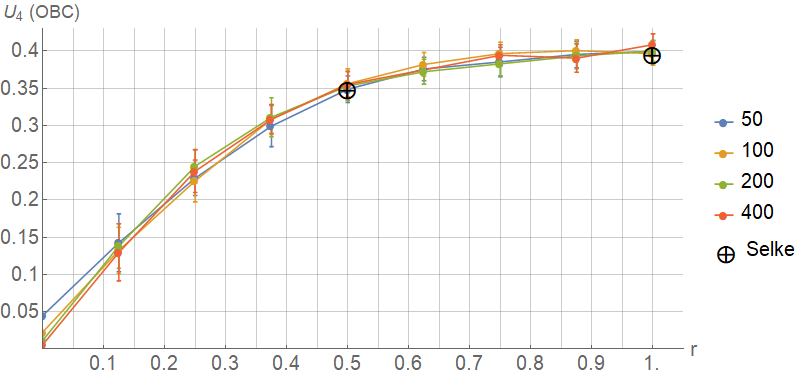
\includegraphics[width=0.5\textwidth]{Images/CumulantOBC.png}
    \caption{Critical cumulant $U_{4}$\eqref{eq:Cumulant} of Ising model on a rectangular lattice with open boundary conditions as function of aspect ratio $r$ with side length $L$ = 50 (blue), 100 (yellow), 200 (green) and 400 (red). Black markers define values from \cite{Selke2006}}
    \label{fig:A_r}
\end{figure} 

By performing Monte-Carlo simulations with steps of Wolff algorithm \cite{Newmanb1999} on Ising model on a rectangular lattice with open boundary conditions in $\theta$-point ($J_{c} = \ln{(1 + \sqrt{2}) / 2} =  0.44068... $), the statistics for Binder cumulant $U_{4}$ were collected with respect to aspect ratio $r$ (see \cref{tab:Ising_T_c}). The results matched with known values from Ref. \cite{Selke2006}.

\begin{figure}[h]
    \centering
    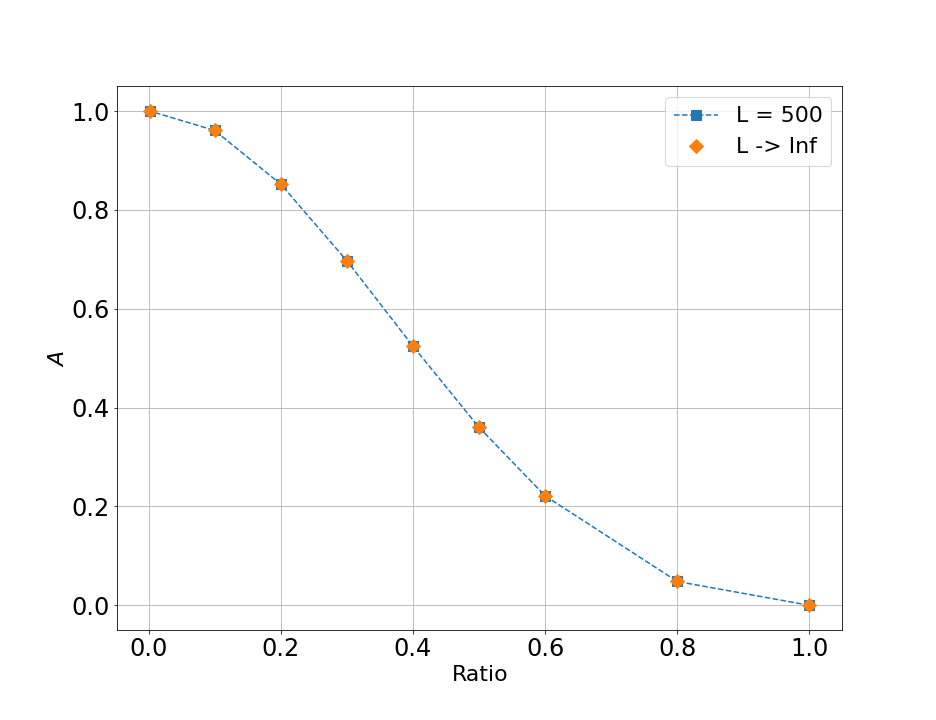
\includegraphics[width=0.5\textwidth]{Images/A_r.png}
    \caption{Asphericity as function of aspect ratio $r$ of the rectangular lattice with side length = 500 and approximate values for rectangular lattice with infinitely long side}
    \label{fig:A_r}
\end{figure}


Ising-ISAW and ISAW models were also simulated on the 2D-square lattice for lengths N = 1000-4900 with the algorithm described in \cite{faizullina2021critical}. 
The simulations were performed for $0 < J < 1$, focusing on areas near the respective critical regions.

\Cref{fig:Ising&ISAW_A_J} shows results of the simulations for asphericity \eqref{eq:Asphericity} as function of J. 
For ISAW model $J_{c} = 0.6673(5)$, and the results are matching to known values from  Ref. \cite{Caracciolo2011}, where critical region was also enumerated.
A critical value of Ising-ISAW model was took from previous work: $J_{c} = 0.8340(5)$ \cite{faizullina2021critical}, while the border critical values depicts results from Ref.\cite{Foster2021} ($J_{c} = 0.8340 \pm 0.0021$). 
Both values were marked as black vertical lines with blue zone around, which will be referred as all statistical errors of critical regions. 
Horizontal line defines value of critical asphericity of ISAW model, which is known from Ref. \cite{Caracciolo2011}, which the results for ISAW model in this paper matches with.

\begin{figure}[h!]
        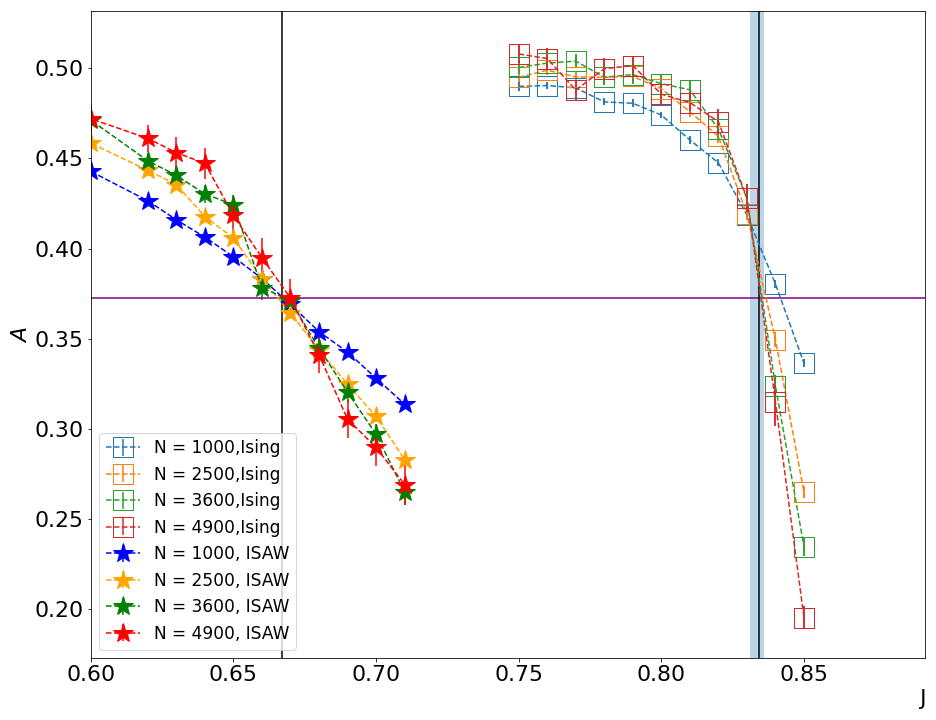
\includegraphics[width=0.5\textwidth]{Images/Ising_ISAW_A_J_Full.png}
        \caption{Asphericity of Ising-ISAW (empty squares) and ISAW-only models (stars) as function of $J=1/T$, varying lengths of conformations $N$ = 1000 (blue), 2500 (yellow), 3600 (green) and 4900 (red)}
        \label{fig:Ising&ISAW_A_J}
\end{figure}
\begin{figure}[h!]
        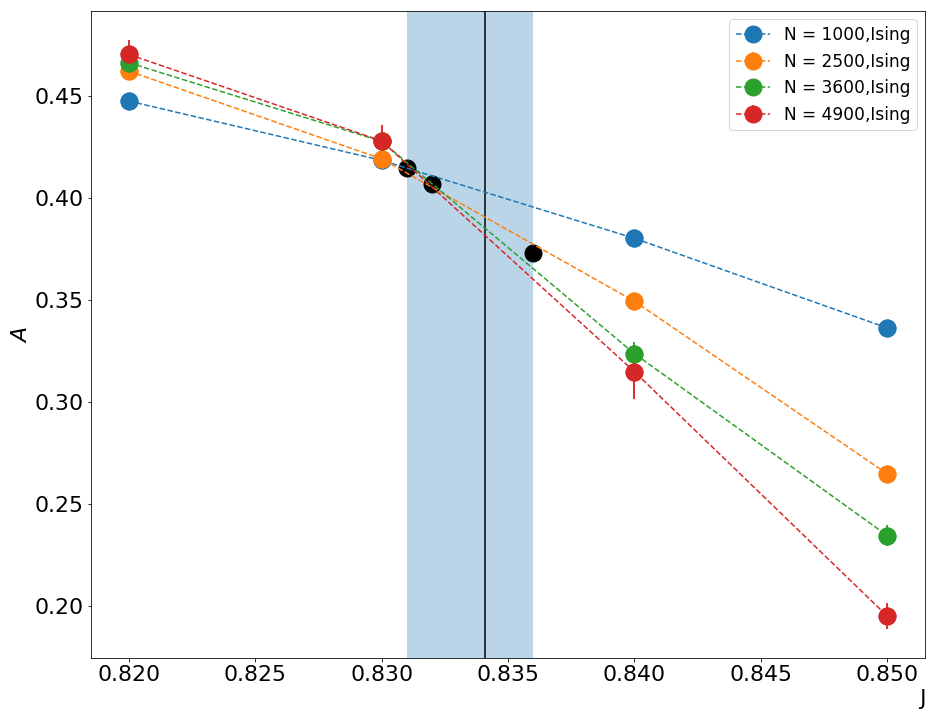
\includegraphics[width=0.5\textwidth]{Images/Ising_A_J_Close.png}
        \caption{Asphericity of Ising-ISAW model as function of zoomed in the critical region (blue zone, according to Ref. \cite{Foster2021} and black vertical line, according to Ref. \cite{faizullina2021critical}), varying lengths of conformations N = 1000 (blue), 2500 (yellow), 3600 (green) and 4900 (red)}
        \label{fig:Ising_A_J}
\end{figure}


The mean values of asphericity of Ising-ISAW model were took in the borders of critical region and in the point of the best crossing of plots where phase transition can be observed according to previous numerical results. All these points are marked as black in zoomed figures \ref{fig:Ising_A_J}. The following steps were to pick up values of aspect ratio, to perform simulations of the Rectangular Ising with the same ratio and, consequently, asphericity and to find critical cumulant of the model with the same shape factors. As it seen from \cref{fig:A_r}, it is enough to use lattice with length $N$ = 500 for picking up the aspect ratio. Simulations were performed with the use of the cluster update based on Wolff algorithm \cite{Newmanb1999} on a rectangular lattice with the same length.\\

\begin{table}[h]
    \centering
    \begin{tabular}{|c|c|c|c|}
        \hline
         \multicolumn{4}{|c|}{Ising-ISAW}  \\ \hline
         J & $\mathcal{A}$ & r & $U_{4}\  Rectangular$ \\ \hline
         0.831 & 0.415 & 0.465 & $0.338 \pm 0.006$\\ \hline
         0.832 & 0.4072 & 0.47 & $0.343 \pm 0.006$\\ \hline
         0.836 & 0.373 & 0.492 & $0.349 \pm 0.006$\\ \hline
         \end{tabular}
    \medskip
    \caption{Values of critical cumulant for Ising model on rectangular lattice with mean asphericity related to Ising-ISAW model in its critical region}
    \label{tab:A_r_U}
\end{table}


As a result, comparison with critical cumulant of Ising-ISAW model, which value was found during simulations in Ref.\cite{faizullina2021critical} ($U_{4} = 0.308(8)$) showed significant mismatch of values, which means that some other geometrical properties might have not been took into account properly - for example, which will be considered in the next part - proportions of monomers with different quantities of nearest neighbors. It is obvious that in Ising model on the rectangular lattice most of monomers are located inside the lattice and have 4 nearest neighbors, while monomers spread around the perimeter of the lattice have only 2 (corners) or 3 nearest neighbors. The proportions in Ising-ISAW conformations are completely different (see \cref{fig:Ising_vs_ISAW2D}).



\subsection{Bulk}

In this section the proportions of monomers with fixed numbers of nearest neighbors for Ising-ISAW and ISAW models on 3D-square and 2D-triangular lattices were studied. 
Monomers of all four modified models can have from 2 to 6 close-range energy connections. 
Some types of monomers, according to number of connections they have, can be interpreted similarly: for example, parts of conformations with monomers with only two nearest neighbors represent 1D-conformations or chains whatever lattice was used in observed model. 
And the opposite - regions where monomers have maximum number of close-range connections represent densely packed areas deep inside the globule. 
In the case of conformations on cubic lattice, other types of monomers can be also interpreted: monomers with only three neighbors define "corners" on conformation, while only monomers on a cube edge (or it also can be on a isolated plane from other part of globule) can have four neighbors. 
Presence of five neighbors belongs to the monomers on a surface of conformation. 
Unfortunately, the similar interpretations cannot be defined for conformations on a triangular lattices.

The first step was to perform simulations of ISAW model on square lattice on lengths from 5 to 3600 at $J=0$ with collecting statistics for fraction of monomers with 2 to 4 neighbors. 
To understand the mechanics of calculating neighbors of monomers, it is required to manually enumerate fractions of monomers with these number of neighbors for short conformations (5 to 11). 
The results of both methods matched.


\subsubsection{Ising model on a SAW-conformation}

Proportions of monomers with 2-6 nearest neighbors in Ising-ISAW model on a three-dimensional square (or cubic) lattice were simulated using method of MC simulations from Ref. \cite{faizullina2021critical}.

As it is seen from left part of \Cref{fig:Ising_vs_ISAW}, increasing the strength of nearest-neighbors interaction J leads to conformation becoming more dense as proportions of monomers with higher numbers of close-range connections significantly increases after $\theta$-transition located in a blue zone (for Ising-ISAW model on a cubic lattice $T_{c} = 0.5263 \pm 0.055$\cite{Foster2021}) (see \Cref{tab:Ising_T_c}).

MC simulations were repeated for two-dimensional triangular lattice. 
Unlike the 3D-square lattice, the 5-th and 6-th possible neighbors located on the same plane as the first four, so conformations are expected to be more dense on this lattice.

The critical region of the model on a triangular lattice was not enumerated yet. 
But as it was suggested, density of conformations becomes higher as nearest-neighbors interaction $J$ strengthen. 
Moreover, the proportion of monomers with six neighbors on a triangular lattice is far higher than on a cubic one. 
It is also significant that "triangular" conformations with no inner interaction have almost twice shorter one-dimensional chains than conformations on a cubic lattice in the same conditions.

\subsubsection{ISAW model}

To understand how the presence of magnetic properties affects on density of models, we also performed Monte-Carlo simulations on a parental model of self-avoiding walks on the same lattices. Results was similar to Ising-ISAW model, as suggested from "parent" model. For cubic lattice $T_{c} = 0.2779\pm 0.0041 $\cite{Tesi1996}. For triangle lattice $J_{c} = 0.405 \pm 0.07 $\cite{Privman1986}. \Cref{fig:Ising_vs_ISAW} shows that geometric aspects of phase transition in ISAW model manifect earlier than in Ising-ISAW ones.  



\subsection{Anticipated results}

Another attactive area of research is zero-interaction zone, where interaction strength J is close to zero and Ising-ISAW and ISAW models converts to non-interacting SAWs.
In previous work \cite{faizullina2021critical}, it was shown that proportion of monomers with 3 neighbours of 2D-square Ising-ISAW model was close to a quarter in zero-interaction zone.
So the following goals of this work are to estimate the scaling nature of SAW models as a functions a length of conformation and the coefficients of scaling functions.
It is expected that the behaviour of triangle SAW will be more close to cubic modification, than to 2D-square version. 


 

\section{Conclusion}

In the first part of the paper we researched critical geometrical properties of Ising-ISAW model on the square lattice, such as mean asphericity of the conformation and aspect ratio. The results were compared with the previous results of research of the Rectangular Ising model, in attempt to find universal magnetic properties in the critical area. The comparison of observed models showed complete dissimilarity of critical bevaviour of magnetic properties between them.

The behaviour of the new metric of compaction of confromation - proportion the monomers with fixed number of the nearest neighbors - was reseacrhed in the second part of the paper. The metric showed clear features of extended and swollen states of conformations between the $theta$-point. The metric also indicates the first-order phase transition for cubic model and the continuous type of transition on the triangle lattice, which clearly correlates this previous results in \cite{Foster2021, faizullina2021critical}

Found differencies between models showed that both models can be equally useful, so they cannot be interchangeable in random walk based algorithms with accent on local coordination number. In sociology both models can be applied as different strategies for analysis of connections in social networks.

Further work can be directed in research another case of local coordination number, such as atmosphere of SAW-conformation, defined as a number of free lattices nodes near the end of conformation.

\bibliographystyle{IEEEtran}
\bibliography{bibliography}

\null \hfill Word count: 2830
\section{Appendices}

\begin{figure*}[]
    \centering
    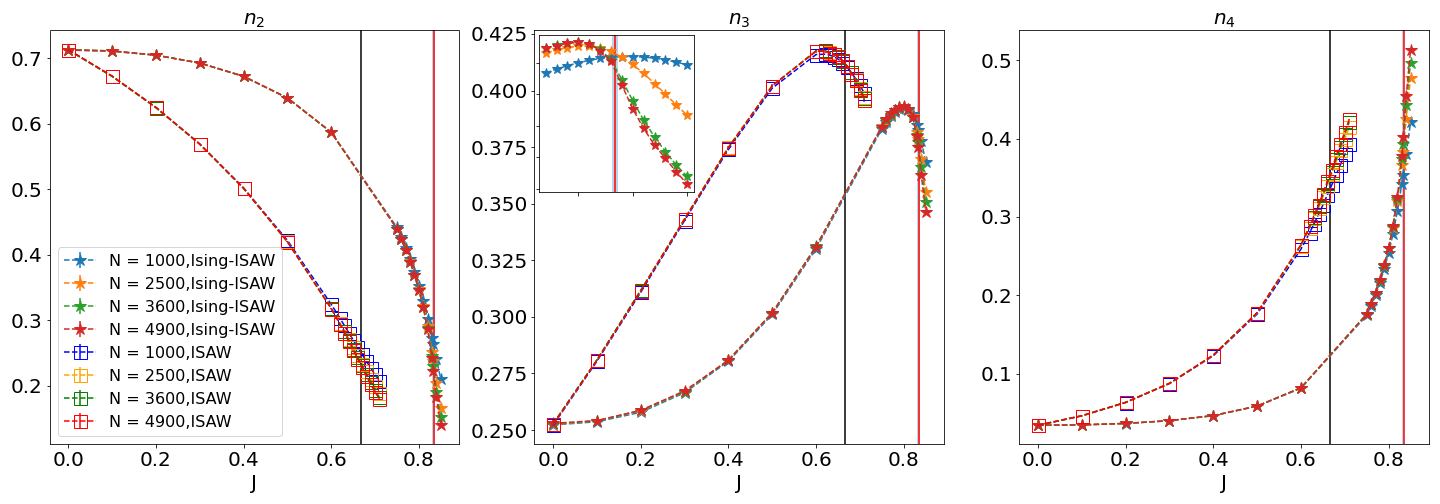
\includegraphics[width=0.99\textwidth]{Images/bulk2-4_inset.png}
    \caption{Fractions of monomers of Ising-ISAW model (squares) and ISAW model (stars) on a square lattice with 2-4 nearest neighbors as function of $J$ with length of conformations $N = $ 1000 (blue), 2500 (yellow), 3600 (green), 4900 (red). Black vertical line define point of $\theta$-transition for ISAW model \cite{Caracciolo2011}, red line - for Ising-ISAW model \cite{faizullina2021critical, Foster2021}. Reproduced from Ref.\cite{faizullina2021critical}}
    \label{fig:Ising_vs_ISAW2D}
\end{figure*}


\begin{figure*}[]
    \centering
    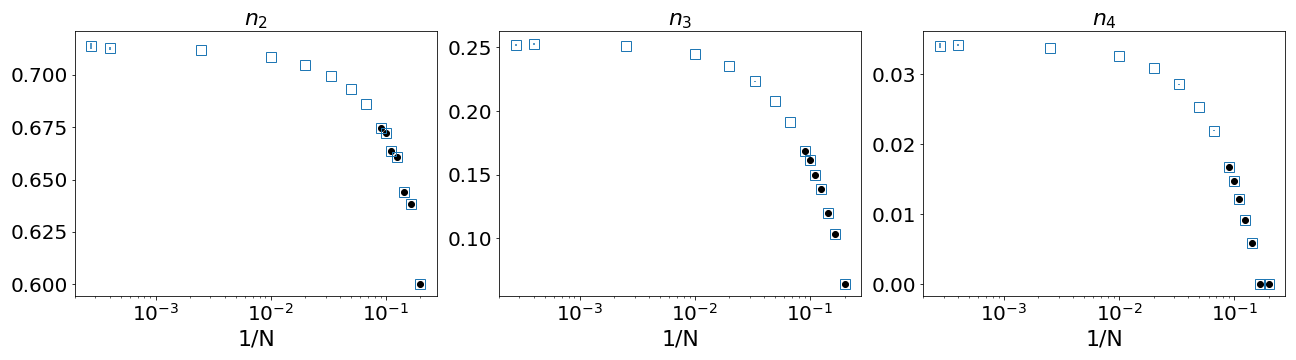
\includegraphics[width=0.99\textwidth]{Images/ISAWJ0_Bulk2-4.png}
    \caption{Fractions of monomers of ISAW model on a square lattice with 2-4 nearest neighbors at $J=0$ as function of $1/N$, from $N = 5$ to $3600$ for MC simulations (empty squares) and from $N = 5$ to $11$ for enumerations (black dots)}
    \label{fig:Ising_vs_ISAW}
\end{figure*}

\begin{figure*}
    \centering
    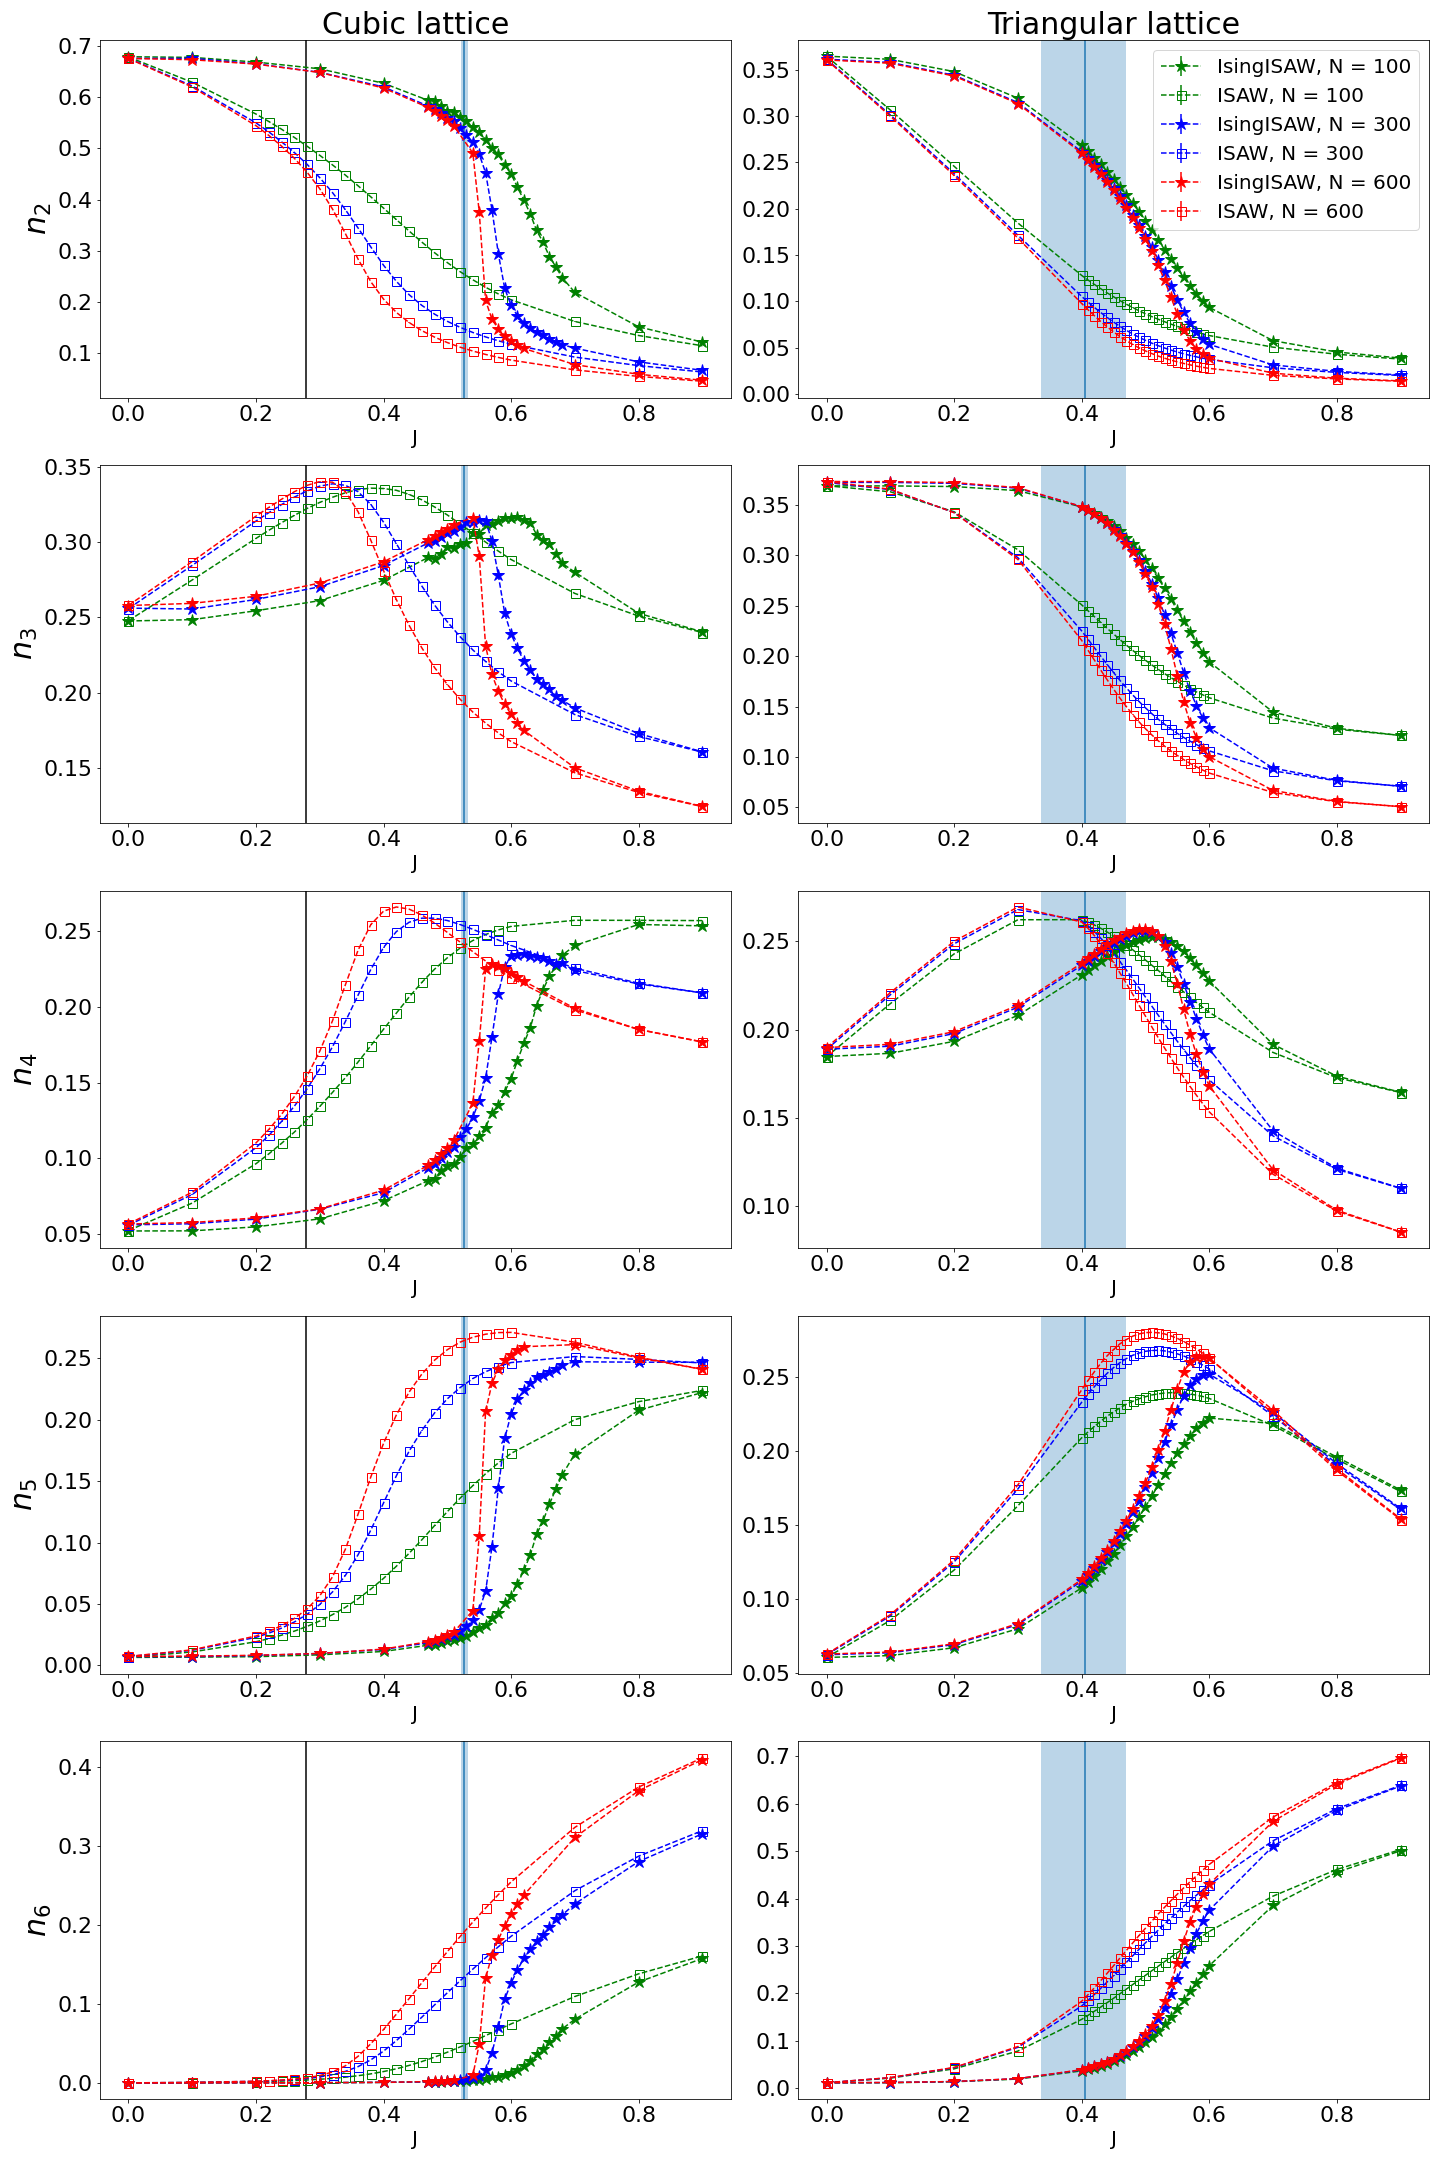
\includegraphics[width=0.95\textwidth, height=22.5cm]{Images/Ising_vs_ISAW.png}
    \caption{Fractions of monomers of Ising-ISAW model (stars) and ISAW model (open squares) on a cubic lattice (left column) and 2D-triangle lattice (right column) with 2-6 nearest neighbors as function of $J$ with length of conformations $N = $ 100 (green), 300 (blue) and 600 (red). Vertical lines define points of $\theta$-transition (For cubic lattice: black line for ISAW model \cite{Tesi1996} and blue line for Ising-ISAW model \cite{Foster2021}; for triangle lattice: blue line for ISAW model \cite{Privman1986})}
    \label{fig:Ising_vs_ISAW}
\end{figure*}

\end{document}